\documentclass{standalone}
\usepackage{tikz}

\begin{document}
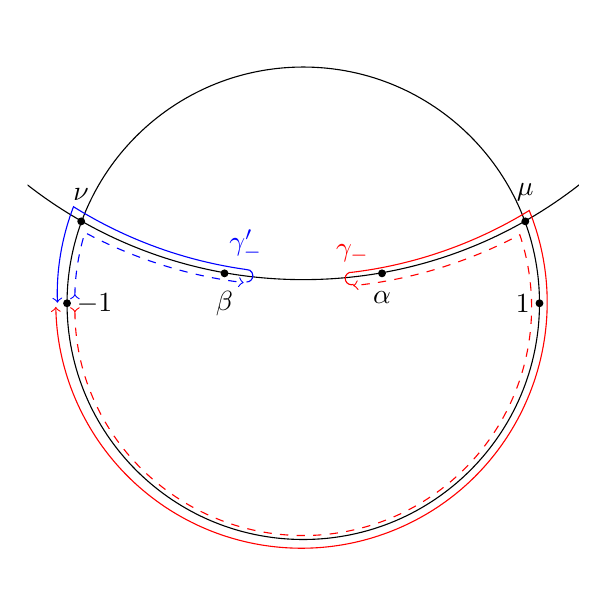
\begin{tikzpicture}
\clip (-3.5,-3.5) rectangle (3.5,3.5);
% \draw[step=0.1,gray,very thin] (-6,-6) grid (6,6);

% unit circle
\draw (0,0) circle [radius=3];
% branch point circle
\draw[color=black] (0,6) circle [radius=5.7];

% γ'_- path, from -1 but around ν
\draw[color=blue,dashed,>->] (-2.9,0.05)
    arc (180:163:2.9)
    arc (-118:-97:5.8);
\draw[color=blue,->] (-0.72,0.27)
    arc (-90:97:0.08)
    node[above, color=blue]{$\gamma'_-$}
    arc (-98:-122:5.6)
    arc (159:182:3.1);

% γ_- path, from -1
\draw[color=red,dashed,>->] (-2.9,-0.05)
    arc (180:378.5:2.9)
    arc (-62:-84:5.8);
\draw[color=red,->] (0.64,0.24)
    arc (-70:-280:0.08)
    node[above, color=red]{$\gamma_-$}
    arc (-83:-58.5:5.6)
    arc (22:-179:3.12);

% γ_- path, from -1
% \draw[color=blue,dashed,>->] (-2.9,0)
%     node[above right, color=blue]{$\gamma_-$}
%     arc (180:74:2.9)
%     arc (-25:-35:7.6)
%     arc (135:315:0.16);
% \draw[color=blue,->] (0.35,1.40)
%     arc (325:337:7.9)
%     arc (68:180:3.1);

% points
\fill (3,0) circle (0.05) node[left, color=black]{$1$};
\fill (-3,0) circle (0.05) node[right, color=black]{$-1$};
\fill (2.82,1.04) circle (0.05) node[above=4, color=black]{$\mu$};
\fill (-2.82,1.04) circle (0.05) node[above=4, color=black]{$\nu$};
\fill (1,0.38) circle (0.05) node[below=3, color=black]{$\alpha$};
\fill (-1,0.38) circle (0.05) node[below=3, color=black]{$\beta$};

\end{tikzpicture}
\end{document}
